\section{K-means algorithm}

Bei der K-means Klassifizierung wird  mit einer Anzahl k, zufällige gewählten Startpunkten, es wird für alle Punkte die Distanz  zu allen k-punkten berechnet. Die Punkte werden dem Startpunkt zugeordnet zu dem sie den geringsten Abstand haben. Für jede Punktmenge wird nun der Mittelpunkt berechnet.Für diese Mittelpunkte führt man die Prozedur dann erneute aus, solange bis eine Anzahl an Max-iterationen erreicht wurde oder die Änderung der Mittelpunkte unter einem gewissem Minimum liegt. 


\begin{figure}[h!]
  \begin{center}
    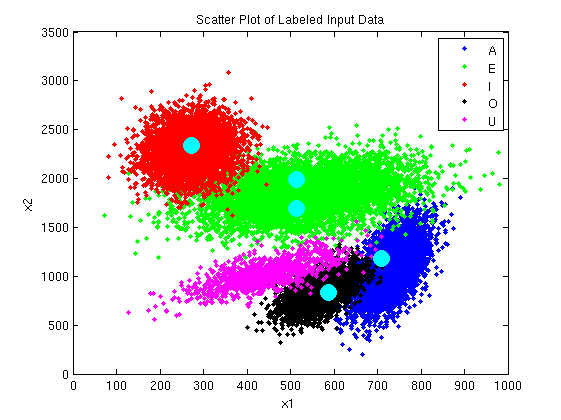
\includegraphics[width=1.0\textwidth]{./figures/6_2_labeled}
    \caption{Die Punktmengen wie sie zugeordnet werden sollten.}
    \label{fig:6_2_labeled}
  \end{center}
\end{figure}

Abbildung~\ref{fig:6_2_labeled} zeigt die Punkte, mit verschiedenen Farben für die verschiedenen Klassen, so wie sie idealer weise klassifiziert werden sollten.


\begin{figure}[h!]
  \begin{center}
    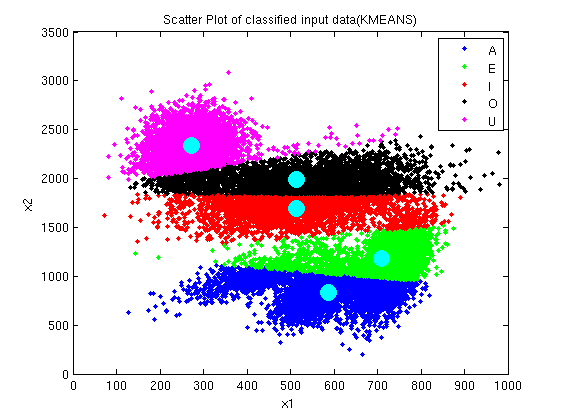
\includegraphics[width=1\textwidth]{./figures/6_2_classified}
    \caption{Mit K-means Klassifiziert.}
    \label{fig:6_2_classified}
  \end{center}
\end{figure}

Abbildung~\ref{fig:6_2_classified} zeigt die Punkte wie Sie mit K-means Klassifiziert werden.\newline
 


Die Klassifizierung von K-means fällt für jedes mal anders aus, das kommt daher da die Klassifizierung von den K-Startpunkte abhängig ist. Um alle Klassen richtig zu finden muss man also mit den Anfangswerten Glück haben (oder man legt die Startpunkte nicht zufällig in den Raum)! Wie man in Abbildung~\ref{fig:6_2_classified} erahnen kann ist die Klassifikation mit K-means für sich schneidende mengen nicht perfekt ist, die Klassifikation erzeugt gerade Schnitte (Abstand zwischen 2 Mittelpunkten).
In unseren Plotts sind die Mittelpunkte von  EM und von K-means sehr ähnlich, nur bei der Klassifizierung wird ein unterschied bemerkbar, da durch die Gauß-verteilung bei EM die Punktwolken angenähert werden und bei K-means nur eine Unterteilung in Zonen stattfindet.